\section{Wechselströme}

\vspace{1\baselineskip}

Da $Q = C V$ folgt: $I = - \frac{dQ}{dt} = -C \frac{dV}{dt}$.

\vspace{1\baselineskip}

\fat{Frei schwindenger gedämpfter $LRC$-Stromkreis}
\begin{itemize}
    \item $\omega_0 = \sqrt{\frac{1}{LC}}$
    \item $\rho = \frac{R}{2L}$
\end{itemize}
\begin{enumerate}
    \item \fat{Schwache Dämpfung}: $\rho^2 < \omega_0^2$ oder $R^2 < 4 \frac{L}{C}$:
            Lösung: $V(t) = V_0 e^{\frac{R}{2L}t} \cos(\omega t)$ \ mit \
            $\omega = \sqrt{\omega_0^2 - \rho^2} = \sqrt{\frac{1}{LC} - \frac{R^2}{4L^2}}$
    \item \fat{Starke Dämpfung}: $\rho^2 > \omega_0^2$ oder $R^2 > 4 \frac{L}{C}$: Lösung:
            $V(t) = A e^{-\beta_1 t} + B e^{- \beta_2 t}$ \ mit \
            $\beta_{1,2} = \frac{R}{2L} \pm \sqrt{\frac{R^2}{4L^2} - \frac{1}{LC}}$
    \item \fat{Sehr starke Dämpfung}: $R^2 >> 4 \frac{L}{C}$: Lösung:
            $V(t) = V_0 e^{- \frac{R}{L} t}$
    \item \fat{Kritische Dämpfung}: $\rho = \omega$ oder $R^2 = 4 \frac{L}{C}$: Lösung:
            $V(t) = A e^{- \frac{R}{2L} t} (1+Bt)$
\end{enumerate}

\vspace{1\baselineskip}

\fat{Zusammenfassung Spannungsabfall}:
\begin{itemize}
    \item Widerstand: $V_R = - I R$
    \item Kondensator: $V_C = \frac{Q}{C}$
    \item Spule: $V_L = - L \frac{dI}{dt}$
\end{itemize}
\fat{Achtung: Vorzeichen sind relativ!}
Beim Kondensator: Ist die Stromrichtung gleich dem Potential\underline{abfall} (von Minus zu
Plus), wo erhalten wir eine parallele Situation. Für die parallele Konfiguration erhalten wir ein
negatives Vorzeichen falls man von \underline{Plus nach Minus} geht! Für den antiparallelen
Fall, haben wir ein positives Vorzeichen.

\vspace{1\baselineskip}

\fat{Verschiedene Stromkreise}:
\begin{itemize}
    \item \fat{$RL$-Stromkreis}: "Strom ist zu Spät, in Induktivität", Lösungen:
            $\tan(\alpha) = - \frac{\omega L}{R}$ und $I_0 =
            \frac{\mathcal{E}_0}{\sqrt{R^2 + \omega^2 L^2}}$
    \item \fat{$RC$-Stromkreis}: "Strom eilt vor, am Kondensator", Lösungen:
            $\tan(\alpha) = \frac{1}{\omega R C}$ und $I_0
            \frac{\mathcal{E}_0}{\sqrt{R^2 + \frac{1}{\omega^2 C^2}}}$
    \item \fat{$RLC$-Schwingkreis}: Lösungen: $\tan(\alpha) = - \frac{\omega L'}{R}$ mit
            $L' = \omega L - \frac{1}{\omega C}$ und $I_0 =
            \frac{\mathcal{E}_0}{\sqrt{R^2 + \klammer{\omega L - \frac{1}{\omega C}}^2}}$

            Maximales $I_0$ bei $\omega_{\text{max}} = \frac{1}{\sqrt{LC}}$.

            Der dimensionslose \fat{Qualitätsfaktor} ist: $\mathcal{Q} = \frac{L \omega_{\text{max}}}{R}
            = \frac{1}{R} \sqrt{\frac{L}{R}}$
\end{itemize}

\vspace{1\baselineskip}

Bei hoher Frequenz des Wechselstromes setzt ein Kondensator dem Stromfluss nahezu keinen
Widerstand entgegen.

\vspace{1\baselineskip}

\fat{Beschreibung durch komplexe Zahlen}:

\begin{itemize}
    \item \fat{elektromotorische Kraft}: $\mathcal{E} (t) = \mathcal{E}_0 e^{i \omega t}$
    \item \fat{komplexe Strom}: $I = I_0 e^{i (\omega t + \alpha)}$
    \item $\alpha = \arctan \klammer{\frac{\Im (I)}{\Re (I)}} =
            \arctan \klammer{\frac{\Im (Y)}{\Re (Y)}}$
    \item \fat{Admittanz}: $Y$: Verallgemeinerung des Leitwertes in Gleichstromkreisen,
            es gilt: $I = Y V$.
    \item \fat{Impedanz}: $Z$: Verallgemeinerung des Ohm'schen Widerstandes, es gilt:
            $Z = \frac{1}{Y} \ \Rightarrow \ V = Z I$.
\end{itemize}

Bei einer \fat{Parallelschaltung} gilt: $Y = \sum_j Y_j$

\vspace{1\baselineskip}

Bei einer \fat{Serienschaltung} gilt: $Z = \sum_j Z_j$

\pagebreak

\begin{center}
    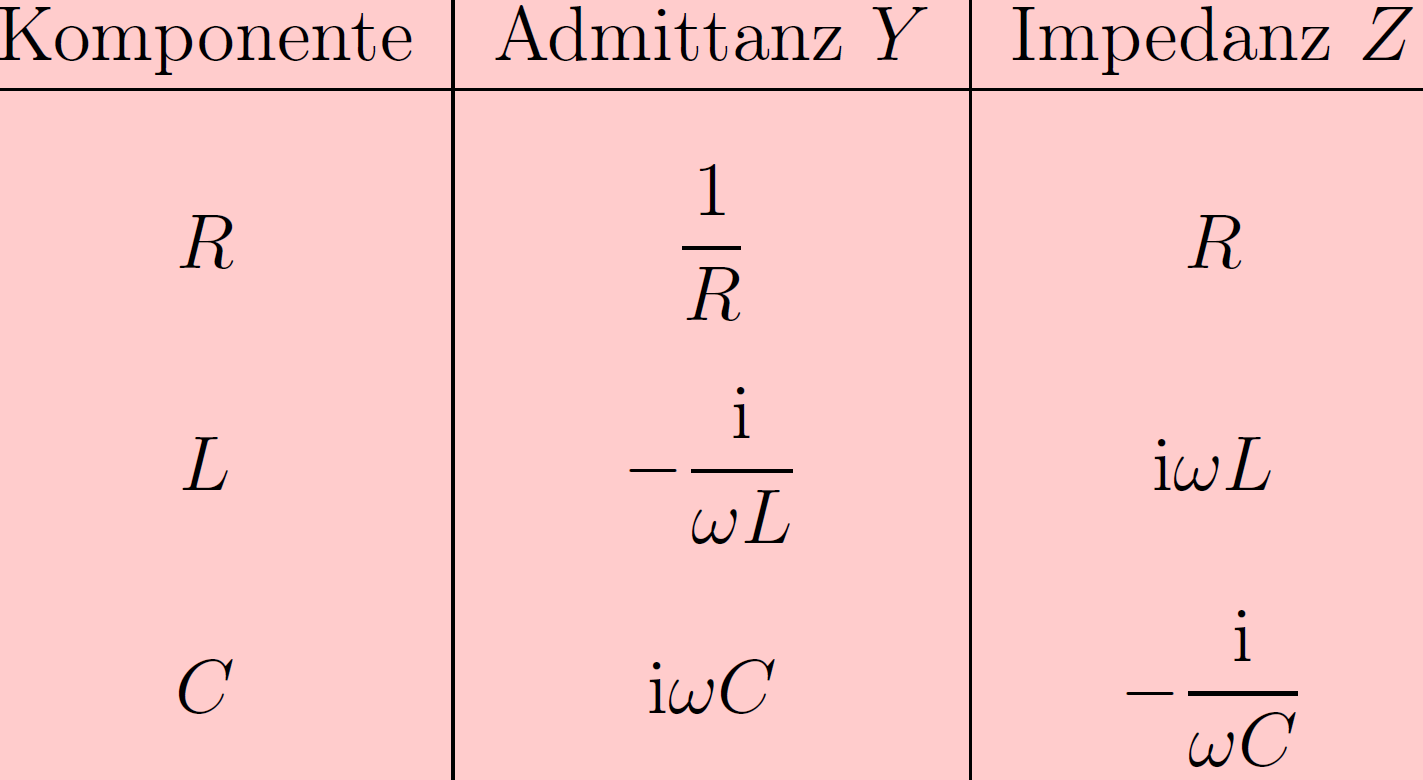
\includegraphics[width=0.3\textwidth]{Figures/Komplex.png}
\end{center}

\vspace{1\baselineskip}

\fat{Leistungsaufnahme eines Stromkreises}

\begin{itemize}
    \item $P = I V$
    \item $\Re (IV) \neq \Re(I) \Re(V)$
    \item Mittlere Leistung: $\langle P \rangle = \langle V I \rangle = \frac{1}{T} \int_0^T V(t) I(t) dt$
    \item \fat{Effektivwerte}: $V_{\text{eff}} = \sqrt{\langle V^2 \rangle}$ und
            $I_{\text{eff}} = \sqrt{\langle I^2 \rangle}$
\end{itemize}
